\subsection{2 ligninger med 2 ubekendte}

I dette delkapitel vil vi gennemgå hvordan man løser 2 ligninger med 2 ubekendte og i hvilket scenario det typisk bliver anvendt.

2 ligninger med 2 ubekendte består af 2 ligninger der hver indeholder 2 variabler. Et eksempel på dette kunne være de følgende 2 ligninger
\begin{align*}
    y = 3x + 4 \hspace{6mm} y = -2x + 4
\end{align*}

Når vi løser 2 ligninger med 2 ubekendte finder vi de værdier for x og y hvor begge sider af lighedstegnet i begge ligninger er ens.

Fremgangsmåden kan beskrives ved følgende steps

\begin{enumerate}
    \item Isoler x i en af de 2 ligninger
    \item Indsæt værdien for x i den anden ligning
    \item Isoler y 
    \item Indsæt y værdien i ligningen hvor x var isoleret
\end{enumerate}

Følger man disse 4 steps finder man værdien for x og y og har dermed løst 2 liginger med 2 ubekendte. For at løse eksemplet ovenfor benytter jeg de 4 steps

Isoler x i den første ligning
\begin{align*}
    y &= 3x + 4\\
    \Updownarrow \hspace{1cm}&\\
    y - 4 &= 3x + 4 - 4 && -4 \hspace{1mm} \text{på begge sider}\\
    \Updownarrow \hspace{1cm}&\\
    y - 4 &= 3x\\
    \Updownarrow \hspace{1cm}&\\
    \frac{y - 4}{3} &= \frac{3x}{3} && \text{Dividerer med 3 på begge sider}\\
    \Updownarrow \hspace{1cm}&\\
    \frac{y - 4}{3} &= x\\
    \Updownarrow \hspace{1cm}&\\
    x &= \frac{y - 4}{3}
\end{align*}

Vi har nu isoleret $x$ i den første ligning. I step 2 indsætter vi værdien for x fra den færste ligning på x's plads i den anden ligning

\begin{align*}
    y &= -2x + 4\\
    \Updownarrow \hspace{2cm}&\\
    y &= -2\cdot \left(\frac{y - 4}{3}\right) + 4 && \text{Indsætter} \hspace{1mm} x = \frac{y - 4}{3}\\
    \Updownarrow \hspace{2cm}&\\
    y - 4 &= -2\cdot \left(\frac{y - 4}{3}\right) + 4 - 4 && -4 \hspace{1mm} \text{på begge sider}\\
    \Updownarrow \hspace{2cm}&\\
    y - 4 &= \frac{-2\cdot (y - 4)}{3}&& \text{Ganger -2 på tælleren}\\
    \Updownarrow \hspace{2cm}&\\
    y - 4 &= \frac{-2y -2\cdot (-4)}{3} && \text{Ganger -2 ind i parentesen}\\
    \Updownarrow \hspace{2cm}&\\
    y - 4 &= \frac{-2y + 8}{3}\\
    \Updownarrow \hspace{2cm}&\\
    (y - 4) \cdot 3 &= \frac{-2y + 8}{3} \cdot 3 && \text{Ganger med 3 på begge sider}\\
    \Updownarrow \hspace{2cm}&\\
    3y - 12 &= -2y + 8 && \text{Ganger 3 ind i parentesen}\\
    \Updownarrow \hspace{2cm}&\\
    3y - 12 + 12 &= -2y + 8 + 12 && +12 \hspace{1mm} \text{På begge sider}\\
    \Updownarrow \hspace{2cm}&\\
    3y + 2y &= -2y + 20 + 2y && +2y \hspace{1mm} \text{på begge sider}\\
    \Updownarrow \hspace{2cm}&\\
    5y &= 20\\
    \Updownarrow \hspace{2cm}&\\
    \frac{5y}{5} &= \frac{20}{5} && \text{Dividerer med 5 på begge sider}\\
    \Updownarrow \hspace{2cm}&\\
    y &= 4
\end{align*}

Step 2 og 3 gav os y værdien $y = 4$. Nu indsætter vi y værdien i den første ligning hvor vi havde isoleret x

\begin{align*}
    x = \frac{y - 4}{3}\\
    \Updownarrow \hspace{1.6cm}&\\
    x = \frac{4 - 4}{3} && \text{Indsæt} \hspace{1mm} y = 4\\
    \Updownarrow \hspace{1.6cm}&\\
    x = 0
\end{align*}

Løsningen til de 2 ligninger er dermed $x = 0$ og $y = 4$. Når vi løser 2 ligninger med 2 ubekendte vil vi typisk få givet 2 lineære funktioner, præcis ligesom eksemplet ovenfor, og når vi så finder x og y værdien har vi faktisk fundet skæringspunktet mellem de 2 linjer. I eksemplet ovenfor vil skæringspunktet derfor være $(0,4)$ og vi kan illustrere dette ved at se på figur \ref{skæring}.

\begin{figure}[ht]
    \centering
    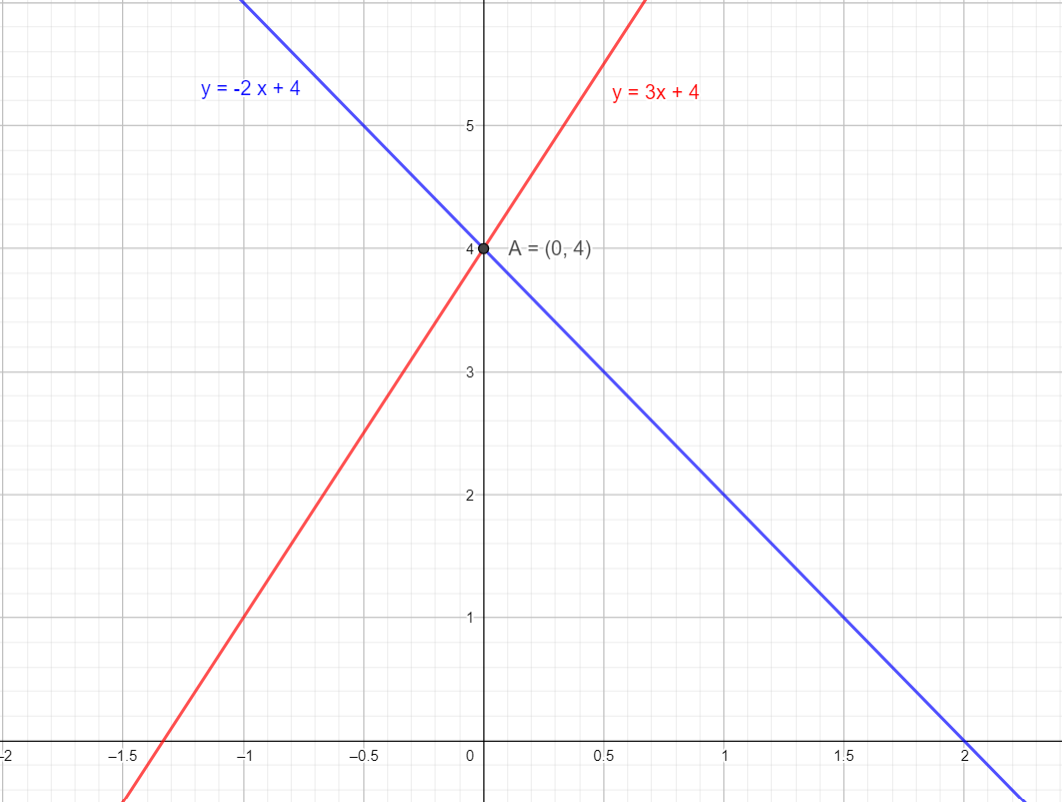
\includegraphics[width=0.8\textwidth]{Figur1}
    \caption{Skæringspunktet mellem 2 linjer}
    \label{skæring}
\end{figure}

Figuren viser de 2 linjer $y = -2x + 4$ og $y = 3x + 4$ og deres skæringspunkt $A = (0,4)$ som var netop det skæringspunkt vi beregnede ved at løse 2 ligninger med 2 ubekendte. 